\documentclass[tikz]{standalone}

\usetikzlibrary{shapes.geometric, arrows}
\tikzstyle{startstop} = [rectangle, rounded corners, minimum width=3cm, minimum height=1cm,text centered, draw=black] % fill=red!30
\tikzstyle{io} = [trapezium, trapezium left angle=70, trapezium right angle=110, minimum width=3cm, minimum height=1cm, text centered, draw=black] % fill=blue!30
\tikzstyle{process} = [rectangle, minimum width=3cm, minimum height=1cm, text centered, text width=3cm, draw=black] % fill=orange!30
\tikzstyle{decision} = [diamond, minimum width=3cm, minimum height=1cm, text centered, draw=black] % fill=green!30
\tikzstyle{arrow} = [thick,->,>=stealth]

\begin{document}
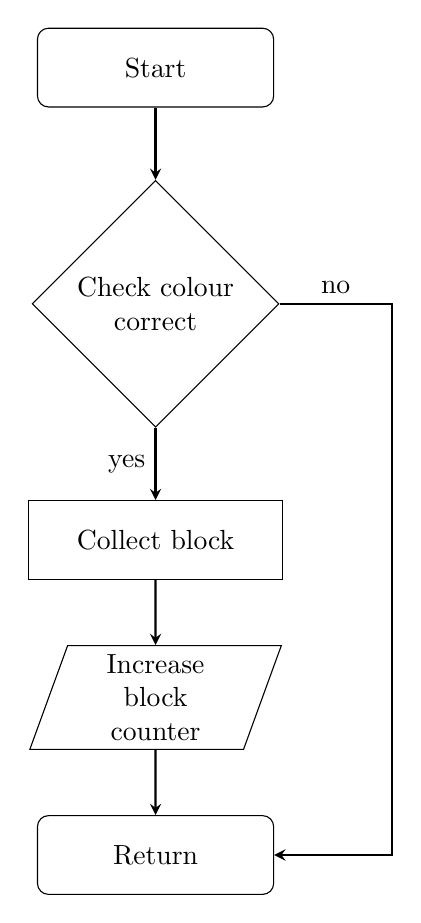
\begin{tikzpicture}[node distance=2cm]
\node (start) [startstop] {Start};

\node (check_color) [decision, below of=start, yshift=-1cm, text width=2cm] {Check colour correct};

\node (collect) [process, below of=check_color, yshift=-1cm] {Collect block};

\node (set_counter) [io, below of=collect, text width=2cm] {Increase block counter};

\node (end) [startstop, below of=set_counter] {Return};



\draw [arrow] (start) -- (check_color); 
\draw [arrow] (check_color) -- node[left] {yes} (collect); 
\draw [arrow] (check_color) -- node[above] {no} ++(3cm, 0) |- (end); 
\draw [arrow] (collect) -- (set_counter); 
\draw [arrow] (set_counter) -- (end); 


\end{tikzpicture}
\end{document}
